\section{Results}\label{sec:results}
Using \fidanka we fit pairs of Population A + E isochrones to the HUGS data for
NGC 2808. Each pair of isochrones is allowed to vary in distance modulus,
reddening, relative helium mass fraction (A/E), and age. Any population pairs which vary by more than 1\% in distance modulus or B-V color excess are rejected. The $\chi^{2}$
distribution for the isochrone pairs is shown in Figure {\color{red}[FIGURE]}.
The best fit isochrones are shown in Figure \ref{fig:BestFitResults} and optimized
parameters for these are presented in Table {\color{red}[TABLE]}.

{\color{red} Need to make the chi2 dist plot still. Have all these values but need to figure out best way to visualize it}

\begin{figure}
  \centering
  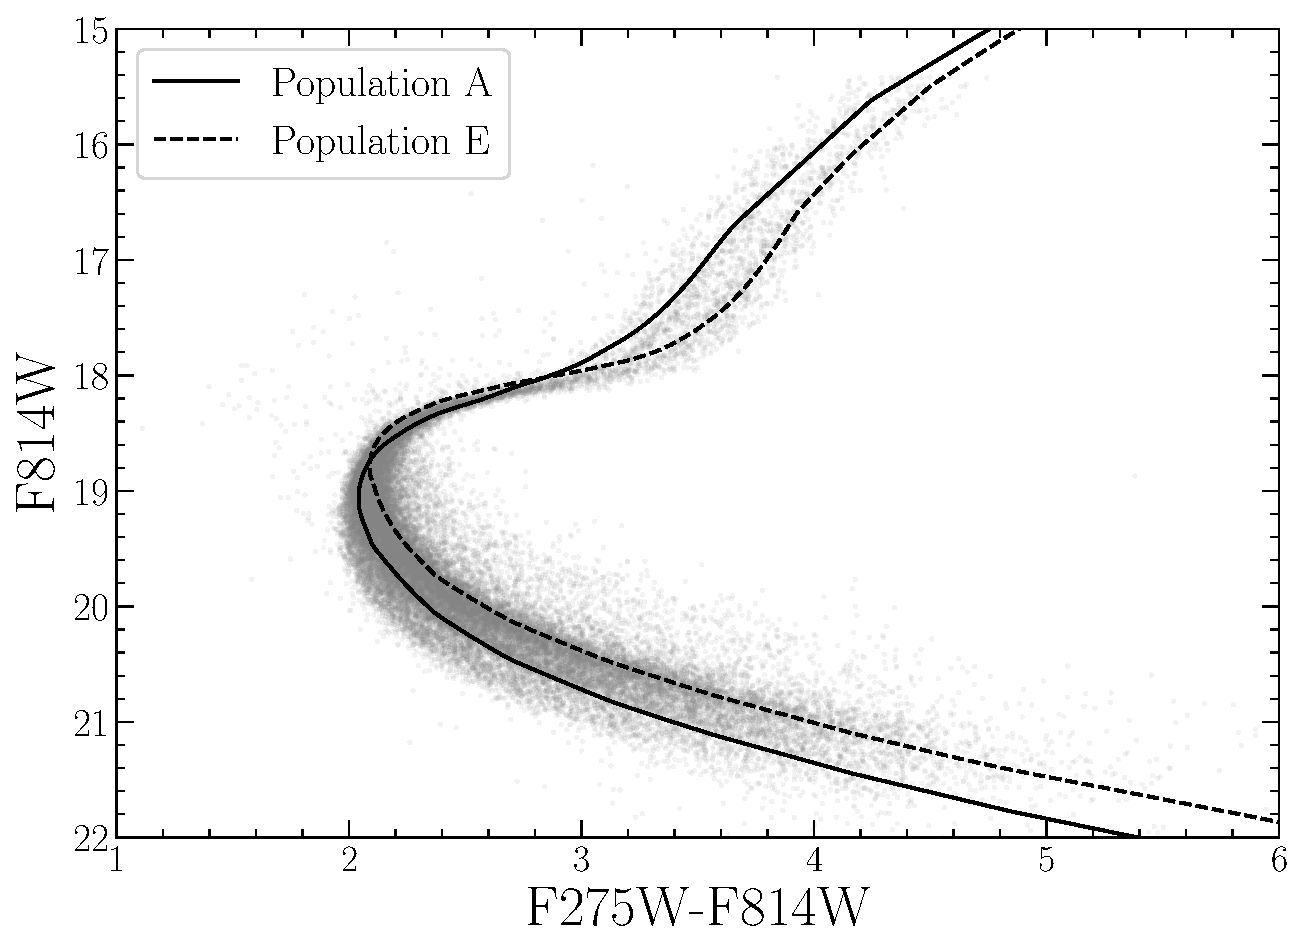
\includegraphics[width=0.45\textwidth]{figures/ngc2808/BestFitResults.pdf}
  \label{fig:BestFitResults}
  \caption{Best fit isochrone results for NGC 2808.}
\end{figure}

\begin{table*}
  \centering
  \begin{tabular}{c | c c c c c c}
    \hline
    population & age & distance modulus & extinction & Y & $\alpha_{ML}$ & $\chi^{2}_{\nu}$\\
    & [Gyr] & & mag & & &\\
    \hline
    \hline
    A & 12.3 & 14.91 & 0.54 & 0.24 & 1.901 & 0.014\\
    E & 14.3 & 14.96 & 0.54 & 0.39 & 1.750 & 0.017 \\
    \hline
  \end{tabular}
  \label{tab:BestFitResults}
  \caption{Best fit parameters derived from fitting isochrones to the fiducual lines derived from the NCG 2808 photometry.}
\end{table*}

{\color{blue} Currently are still seeing a discontinutiy in the isochrobne below the MSTO. This must be addressed before submission.}

\subsection{The Number of Populartions in NGC 2808}
\fidanka provides a somewhat straigtforward way to estimate the number of populations expected in a given magnitude bin given the observations. See Section \ref{sec:fidanka} for specific implimentaiton details. Here we preform an analysis of the number of populations seen in the NGC 2808 F814W-F274W vs F814W color-magnitude diagram. We find that for the majority of the main sequence and red giant branches BGMM prefers two populations; wherease, near the main sequnce turn off and on the majority of the subgiant branches BGMM prefers a single population model.

{\color{red}[FIGURE SHOWING BGMM population probability]}

